\subsection{Serverseitige Architektur}

\subsubsection{Skriptsprachen}

PHP, Python, Ruby, Node.js

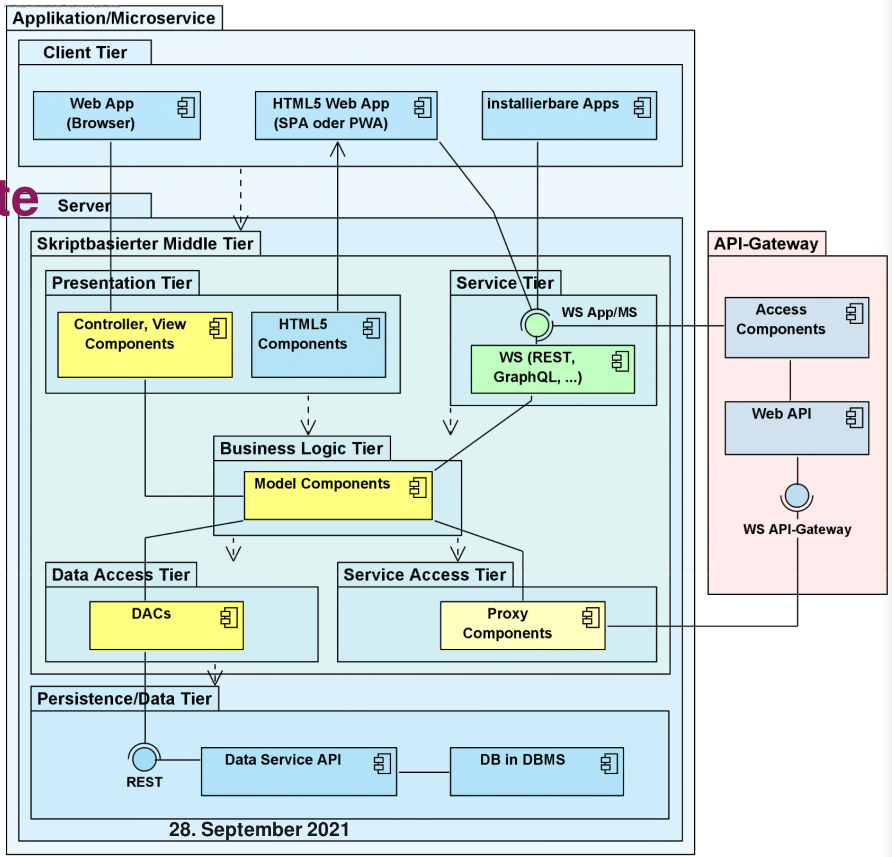
\includegraphics[width=\linewidth]{servers-reference-full-stack.png} \\

\subsubsection{node.js Architektur}

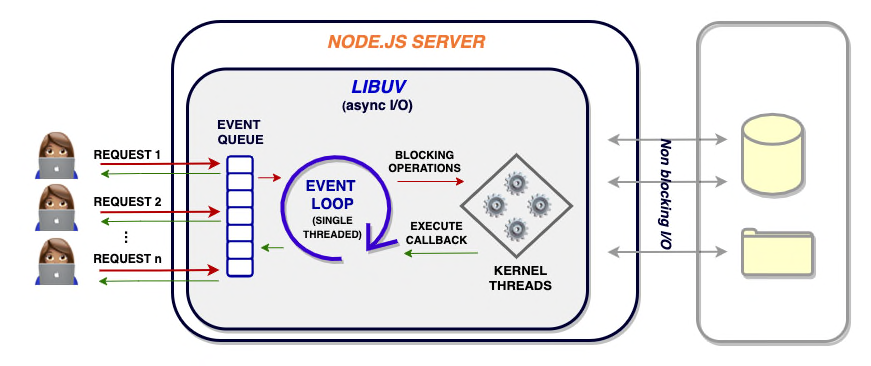
\includegraphics[width=\linewidth]{servers-nodejs.png} \\

\textbf{Mikroarchitektur}

eines Microservice

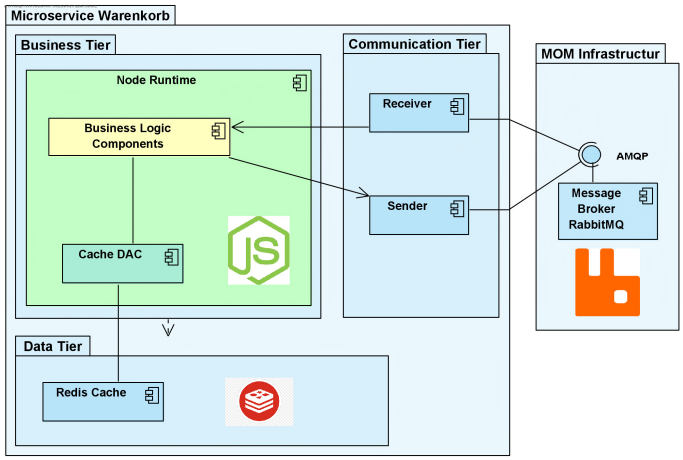
\includegraphics[width=\linewidth]{servers-example.png}

asynchrone Kommunikation, Cache-DB

\subsubsection{.NET Architektur}

\textbf{Merkmale}

Mehrere Programmiersprachen

\begin{itemize}
    \item \textcolor{blue}{C\#} C sharp, objektorientiert, ähnlich wie Java
    \item \textcolor{blue}{VB} Visual Basic
    \item \textcolor{blue}{F\#} funktionale Programmiersprache
\end{itemize}
\vspace{10pt}
Client-Tier

\begin{itemize}
    \item \textcolor{blue}{UX} User Experience
    \item \textcolor{blue}{UWP} Universal Windows App
    \item \textcolor{blue}{Xamarin} Multiplattform Mobile Apps
\end{itemize}
\vspace{10pt}
Web-Tier

realisiert mit IIS, Apache, NGINX und in-memory Kestrel

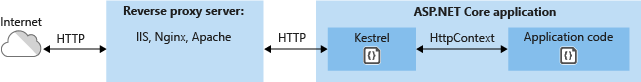
\includegraphics[width=\linewidth]{servers-dotnet-web-tier.png}

Web App

\begin{itemize}
    \item \textcolor{blue}{ASP.NET} Active Server Pages
\end{itemize}
\vspace{10pt}
Data Access

\begin{itemize}
    \item \textcolor{blue}{ORM} Obect-Relational Mapping, Entity Framework
    \item \textcolor{blue}{ODBC} Open Database Connectivity – direkt mit SQL!
    \item \textcolor{blue}{LINQ} Language Integrated Query
    \item \textcolor{blue}{ADO.NET} Active Data Object
\end{itemize}
\vspace{10pt}
\textbf{Full Stack .NET}

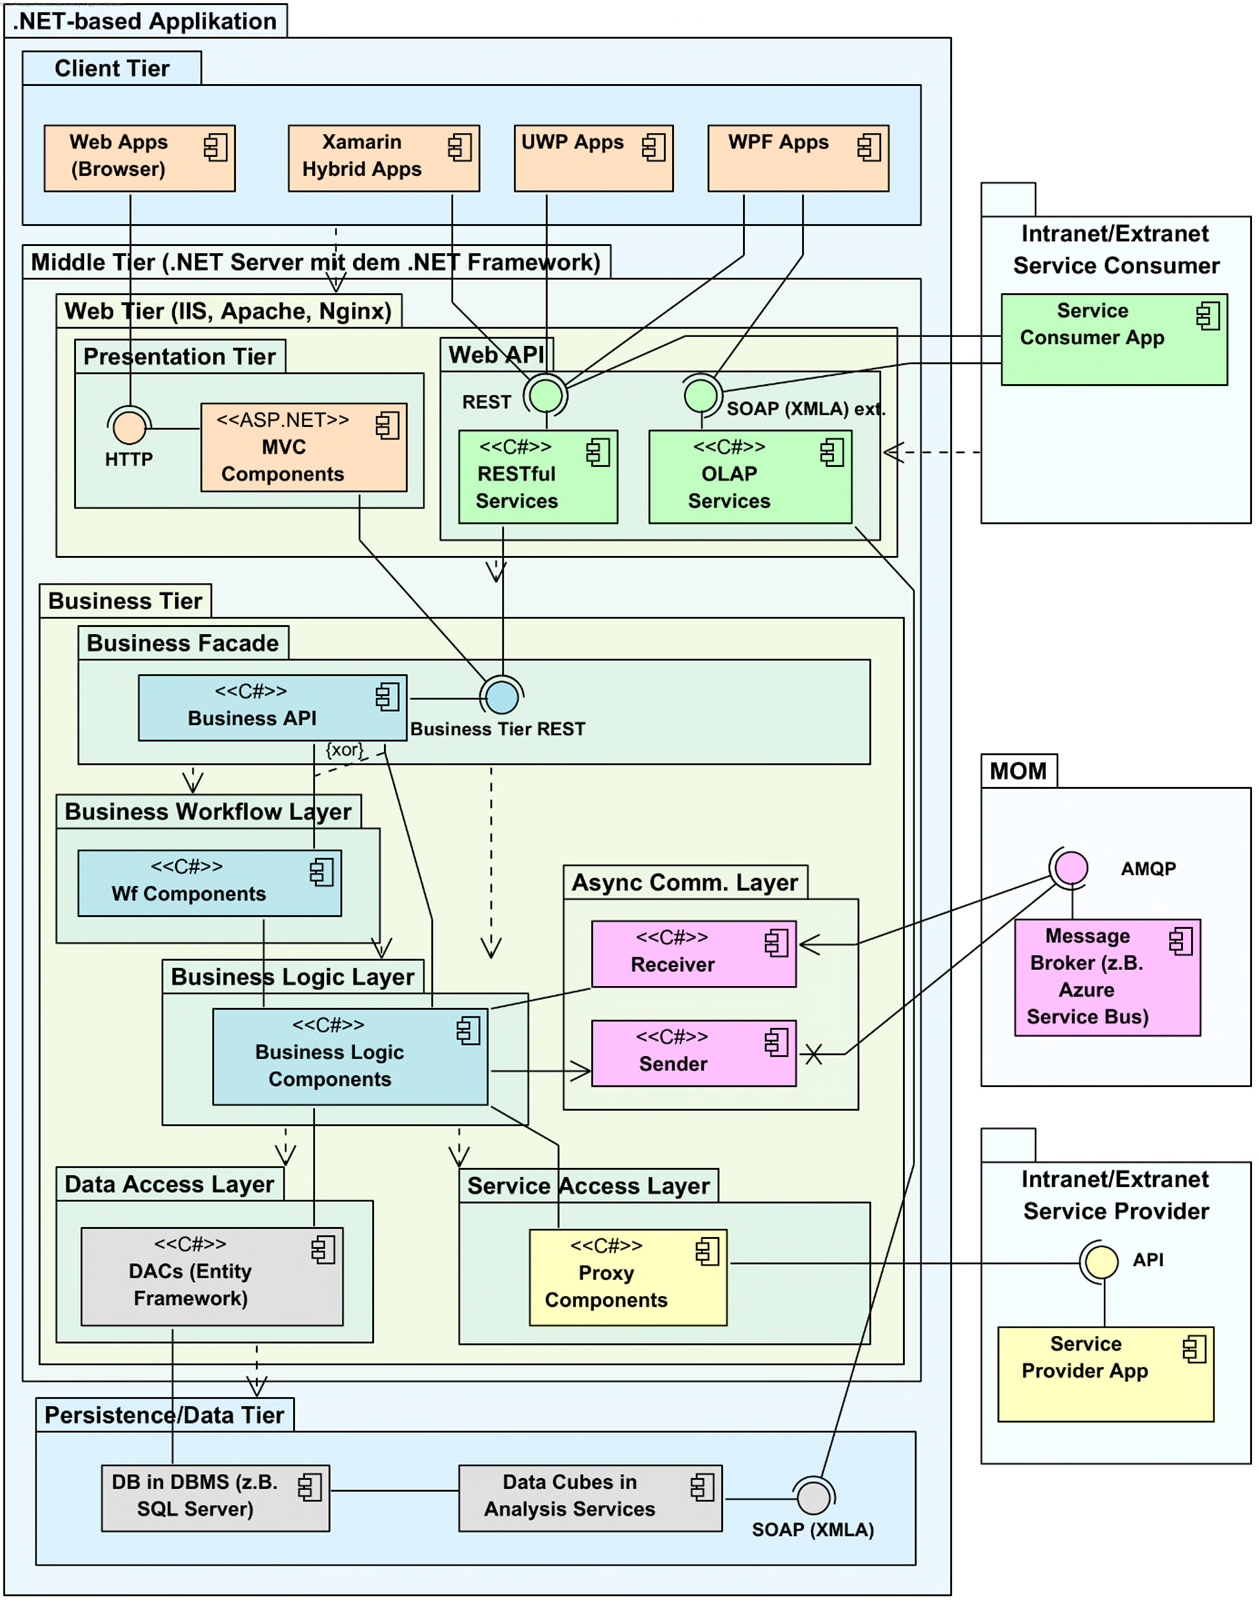
\includegraphics[width=\linewidth]{servers-dotnet-reference.png}

\textbf{Mikroarchitektur}

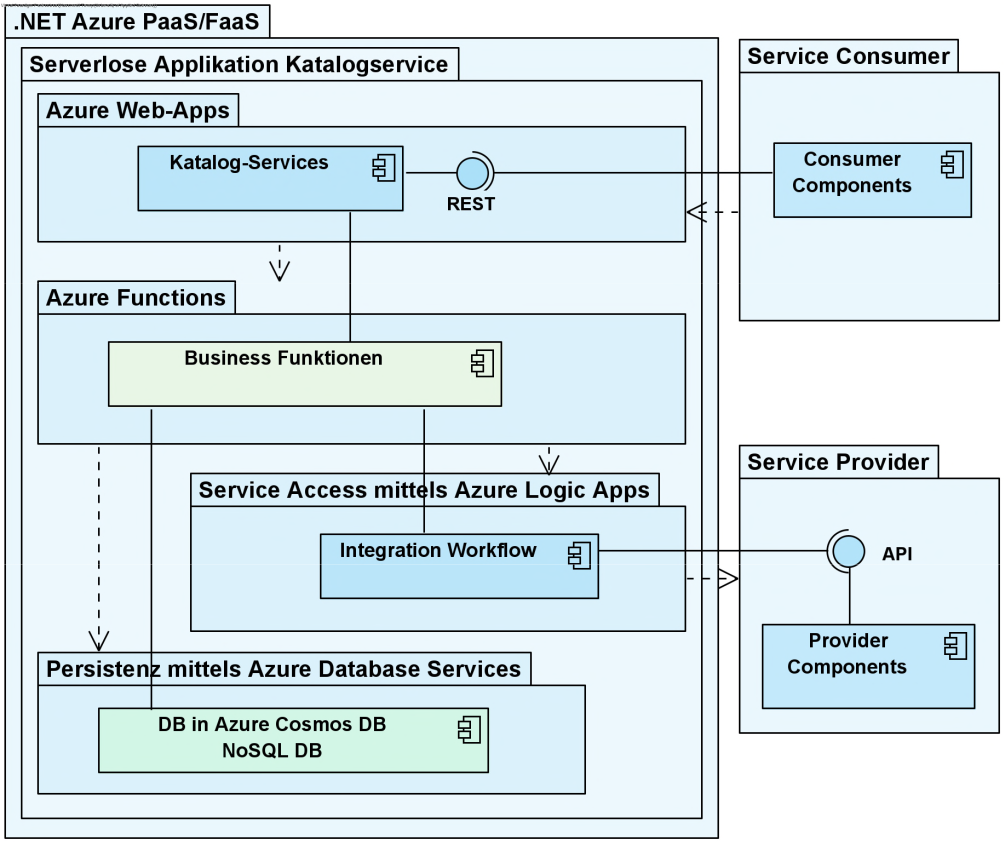
\includegraphics[width=\linewidth]{servers-dotnet-micro.png}

\begin{itemize}
    \item Zugriff erfolgt über eine REST-Schnittstelle, die mit einer Azure Web-App entwickelt ist
    \item Fachlichen Funktionen sind als Azure Functions umgesetzt $\rightarrow$ diese kommunizieren asynchron über den Azure Service Bus
    \item dokumentorientierte Cosmos DB hält die Daten persistent
    \item Azure Logic Apps realisiert die Integration mit den Service Providern
\end{itemize}

\subsubsection{Jakarta EE}

\textbf{Merkmale}

\begin{itemize}
    \item Open Source/Community – geführt von Eclipse
    \item Eine standardisierte Programmiersprache
    \item Web-/Application-Container übernehmen diverse Funktionalitäten/Dienste
    \item viele Anbieter von Web- und Applicationserver
    \item viele IDE's (Integrated Development Environments)
\end{itemize}
\vspace{10pt}
Presentation Layer mit Web App Framework

\begin{itemize}
    \item \textcolor{blue}{JSF} JavaServer Faces, mit EL (Expression Language), Zugriff auf Methoden des Backing Bean
    \item \textcolor{blue}{Backing Bean} Java Klasse, hat Zugriff auf EJBs
\end{itemize}
\vspace{10pt}
Zugriff auf Persistenz (DB)

\begin{itemize}
    \item \textcolor{blue}{JPA} Java Persistence API $\rightarrow$ ORM Object Relational Mapping
    \item \textcolor{blue}{Entity Beans} objektrelationale Abbildung der SQL-DB
    \item \textcolor{blue}{JDBC} Java Database Connectivity (direkt mit SQL)
\end{itemize}
\vspace{10pt}
Applikationsserver

\begin{itemize}
    \item Apache TomEE
    \item GlassFish
    \item Oracle WebLogic
    \item IBM WebSphere
    \item WildFly
\end{itemize}
\vspace{10pt}
JRMP – Java Remote Method Invocation Protocol

\begin{itemize}
    \item \textcolor{blue}{RMI} Remote Method Invocation
    \item \textcolor{blue}{IIOP} Internet Inter ORB [Object Request Broker] Protocol
\end{itemize}

\textbf{Frameworks}

\begin{itemize}
    \item Spring/Spring Boot
    \item Jakarta EE
    \item Hadoop
    \item Play
    \item Grails
    \item Quarkus
\end{itemize}


\textbf{Container-Architektur}

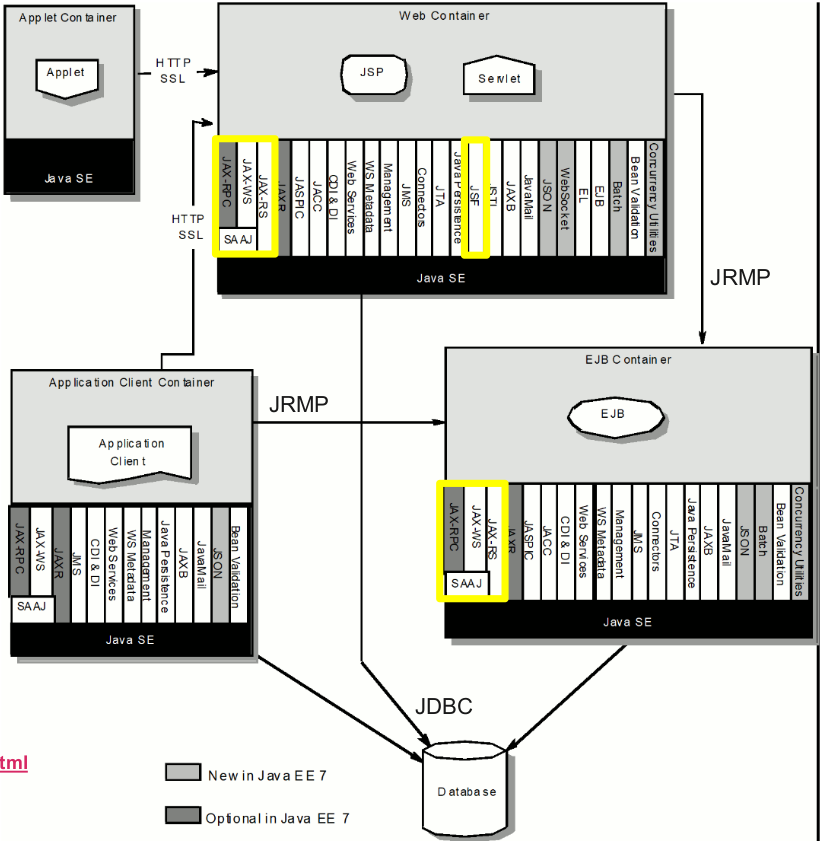
\includegraphics[width=\linewidth]{servers-container.png} \\
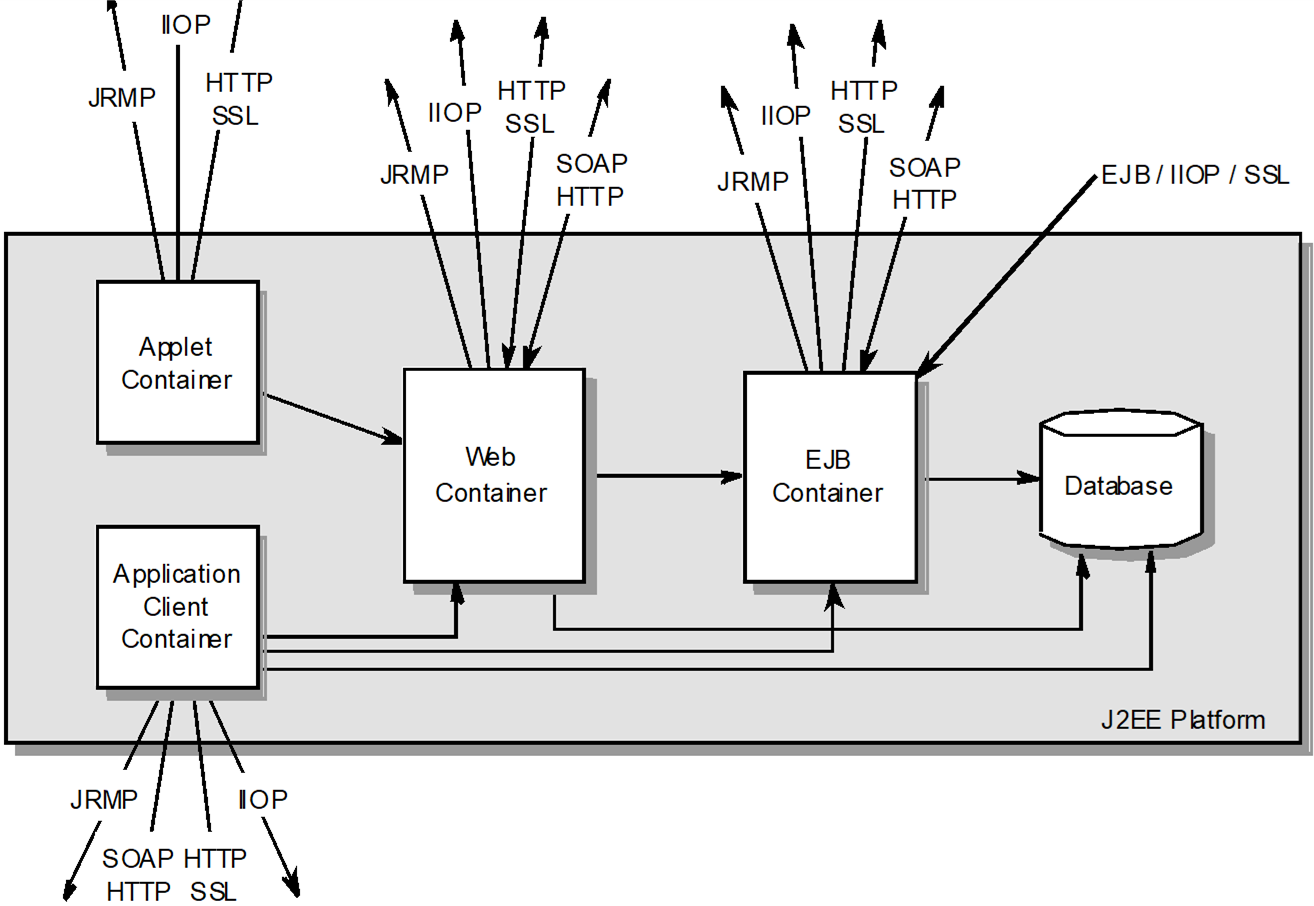
\includegraphics[width=\linewidth]{servers-java-container.png} \\

Client

\begin{itemize}
    \item Applet Container
    \item Application Client Container
\end{itemize}
\vspace{10pt}
Server

Web Container / Web API (Application Programming Interface)

\begin{itemize}
    \item Web Services (REST oder SOAP)
    \item Web Tier
    \item bildet Schnittstelle zum Client Tier bzw. zu den Service Consumer
\end{itemize}
\vspace{10pt}
EJB-Container (Enterprise Java Bean)

\begin{itemize}
    \item Business Tier
    \item hält Geschäftslogik
    \item gehostet in Application Server
    \item Funktionen für das Software Lifecycle Management
    \item Instanziierung, Kontrolle und Skalierung der EJBs (Enterprise Java Beans) $\rightarrow$ EJB sind auf dem Server ausführbare Klassen
    \item \textcolor{blue}{Session Beans (sync)} Stateful, Stateless, Singleton
    \item \textcolor{blue}{Message Driven Bean (async)} mittels JMS (Java Message Service)
\end{itemize}
\vspace{10pt}
\textbf{Makroarchitektur}

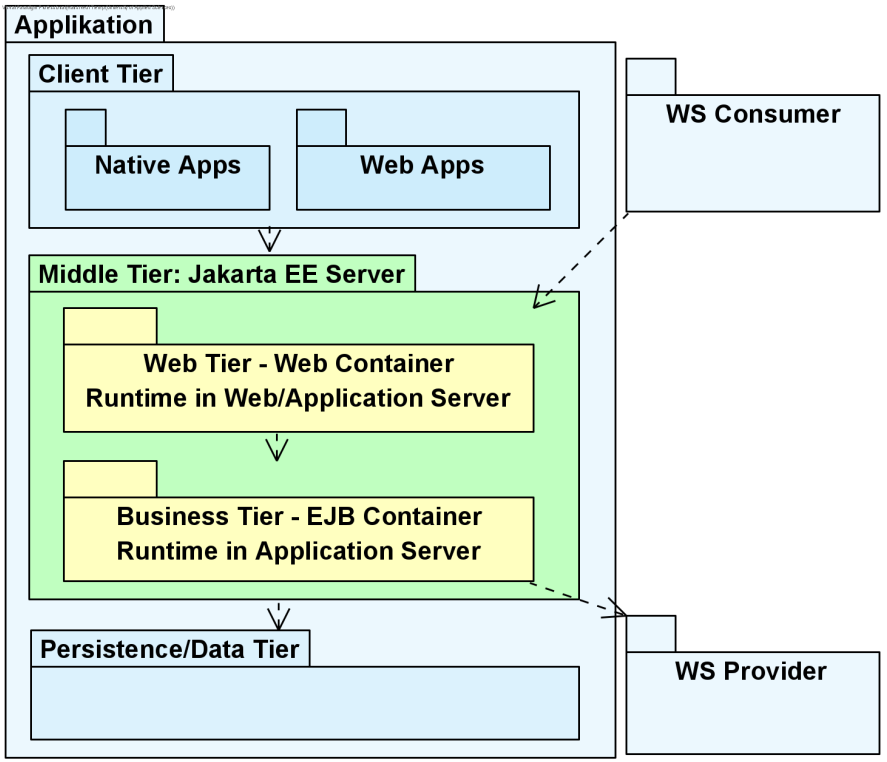
\includegraphics[width=\linewidth]{servers-java-macro.png} \\

\textbf{Mikro-/Referenzarchitektur}

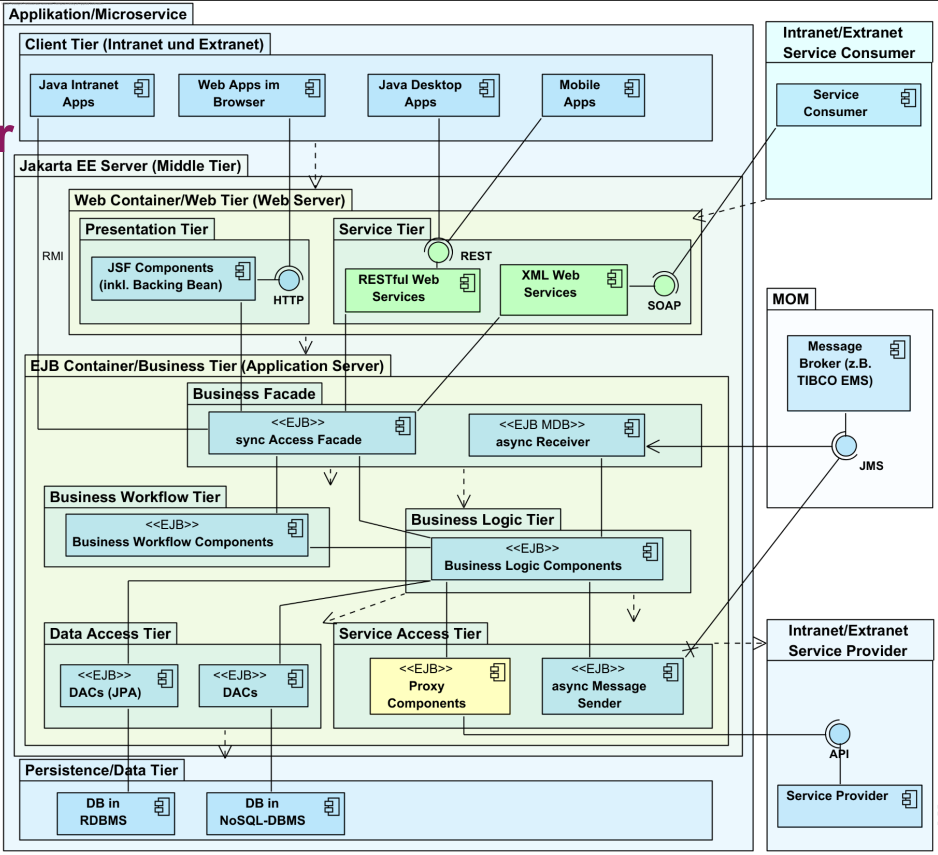
\includegraphics[width=\linewidth]{servers-java-reference.png} \\

\textbf{Example}

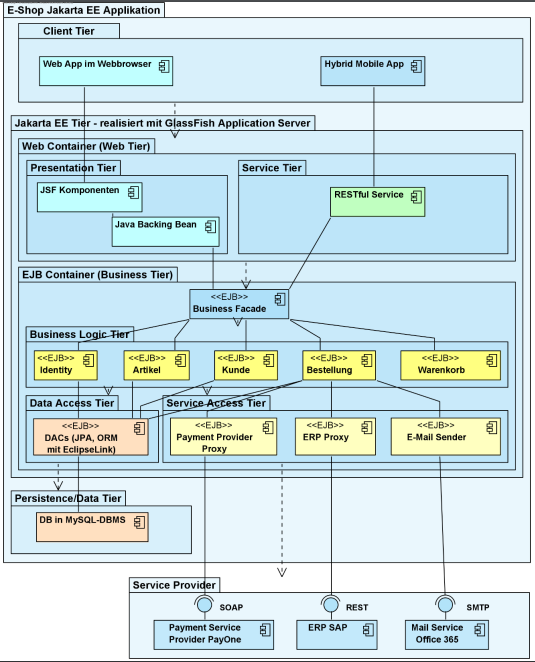
\includegraphics[width=\linewidth]{servers-java-example.png} \\

\textbf{Cloud}

Grundbausteine in AWS

IaaS, PaaS/FaaS

\subsubsection{IoT}
verbindet physische Objekte mit der virtuellen Welt. Intelligente Geräte und Maschinen sind dabei miteinander und mit dem Internet vernetzt. Sie erfassen relevante Informationen über ihre unmittelbare Umgebung, analysieren diese und verknüpfen sie.

\textbf{Cyberphysical (Smart) Things}

Ambient Intelligence

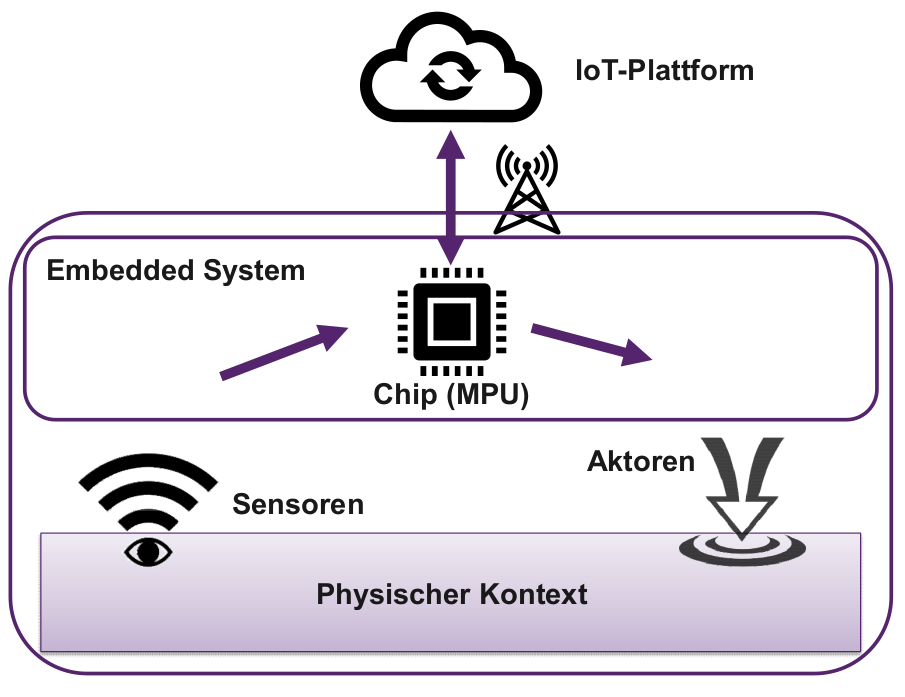
\includegraphics[width=\linewidth]{servers-iot-smart-thing.png}

Ein technisches Gerät, dessen Funktionalitäten und herausragende Eigenschaften sich aus dem vernetzten Zusammenspiel von rechnerischen und physischen Komponenten ergeben. Die CPS-Technologie zielt darauf ab, die für die nahtlose Integration von Cyber- und physischen Systemen erforderlichen Prozesse, Netzwerke und Technologien zu entwickeln

\begin{itemize}
    \item Intelligente Lampe
    \item Smarter Kühlschrank
    \item Smartes Fahrrad
    \item Produktionsmaschine
\end{itemize}
\vspace{10pt}
\textbf{Industrie 4.0}

Vernetzung auf Basis von Cyber-Physical System, intelligente Vernetzung von Maschinen und Abläufen in der Industrie mit Hilfe von Informations- und Kommunikationstechnologie

\textcolor{blue}{RAMI 4.0}
Referenzarchitekturmodell Industrie 4.0

\begin{itemize}
    \item grundlegende Architektur für Industrie 4.0 unter Verwendung eines ausgeklügelten Koordinatensystems
    \item explizite Berücksichtigung des Lebenszyklus von Assets oder Gegenständen im Produktionsumfeld (erlaubt auch immaterielle Objekte)
\end{itemize}

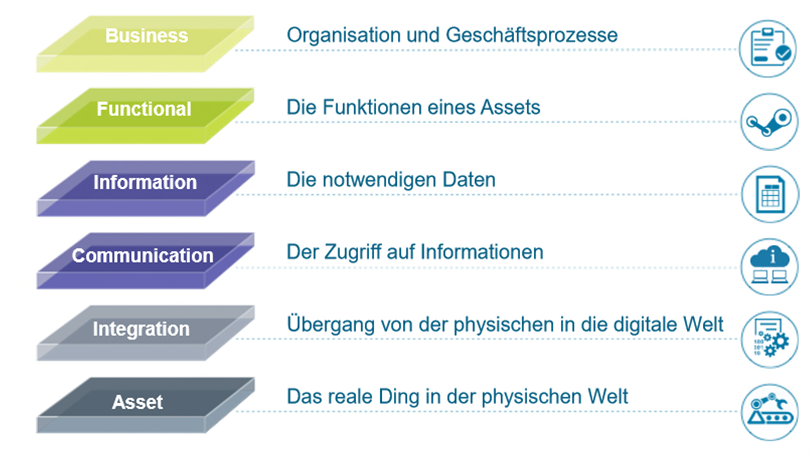
\includegraphics[width=\linewidth]{servers-iot-rami-1.png}

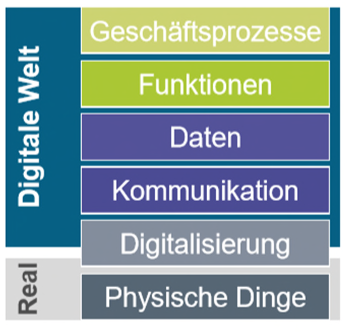
\includegraphics[width=0.5\linewidth]{servers-iot-rami-2.png} \\

\textcolor{blue}{IIRA}

Industrial Internet Reference Architecture

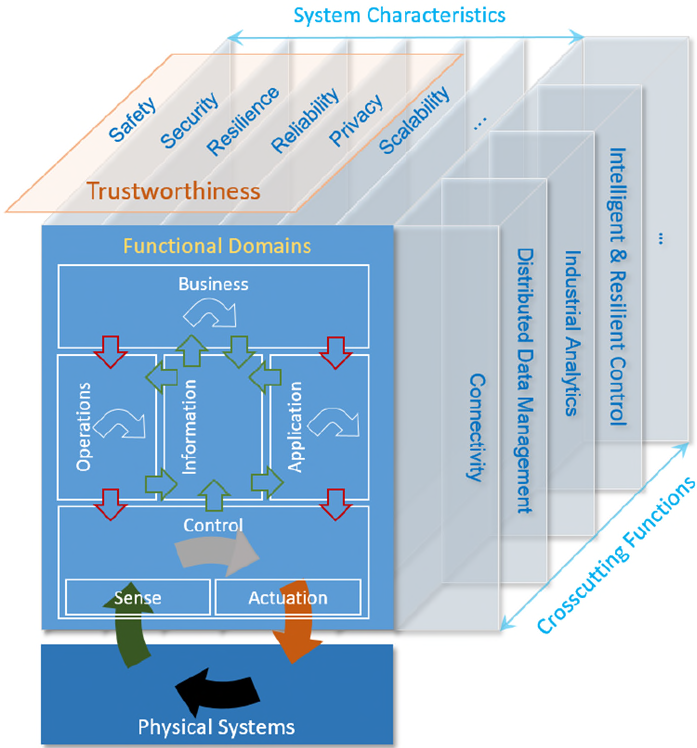
\includegraphics[width=\linewidth]{servers-iot-iira.png}

\begin{itemize}
    \item \textcolor{blue}{business viewpoint} stellt den Bezug zwischen den Belangen der Stakeholder und ihrer unternehmerischen Ziele, Werte und Absichten und dem IIS im Zusammenhang im geschäftlichen und regulatorischen Kontext dar. Diese Belange sind geschäftsorientiert und etwa für Entscheider, Produktmanager und System-Ingenieure von Belang.
    \item \textcolor{blue}{usage viewpoint} skizziert die erwartete Anwendung des Systems. Gewöhnlich wird dieser Sichtpunkt als eine Abfolge von Aktivitäten von menschlichen oder logischen Nutzern dargestellt, die so die angestrebte Funktionalität herstellen und die Fähigkeiten des Systems bereitstellen und ausführen.
    \item \textcolor{blue}{functional viewpoint} legt den Fokus auf die funktionalen Komponenten des IIS, ihre Beziehung zueinander, ihre Struktur, ihre Schnittstellen, ihr Zusammenwirken und den Bezug und die Interaktion des Systems mit externen Bestandteilen, die das Gesamtsystem unterstützen oder erweitern.
    \item \textcolor{blue}{implementation viewpoint} enthält die Techniken, die nötig sind, um die funktionalen Bestandteile zu implementieren, ihre Kommunikation zu ermöglichen und die Abläufe im Lebenszyklus sicherzustellen.
\end{itemize}
\vspace{10pt}
\textbf{Referenzarchitektur}

\begin{itemize}
    \item \textcolor{blue}{Edge Tier} Bereich, in welchem die stationären oder mobilen IoT Devices verortet sind
    \item \textcolor{blue}{Platform Tier} Serverbereich, in welchem sich die Daten und Software zur IoT-Lösung befinden
    \item \textcolor{blue}{Enterprise Tier} beinhaltet alle operativen Fachanwendungen, wie z.B. ERP, CRM, PLM usw.
\end{itemize}

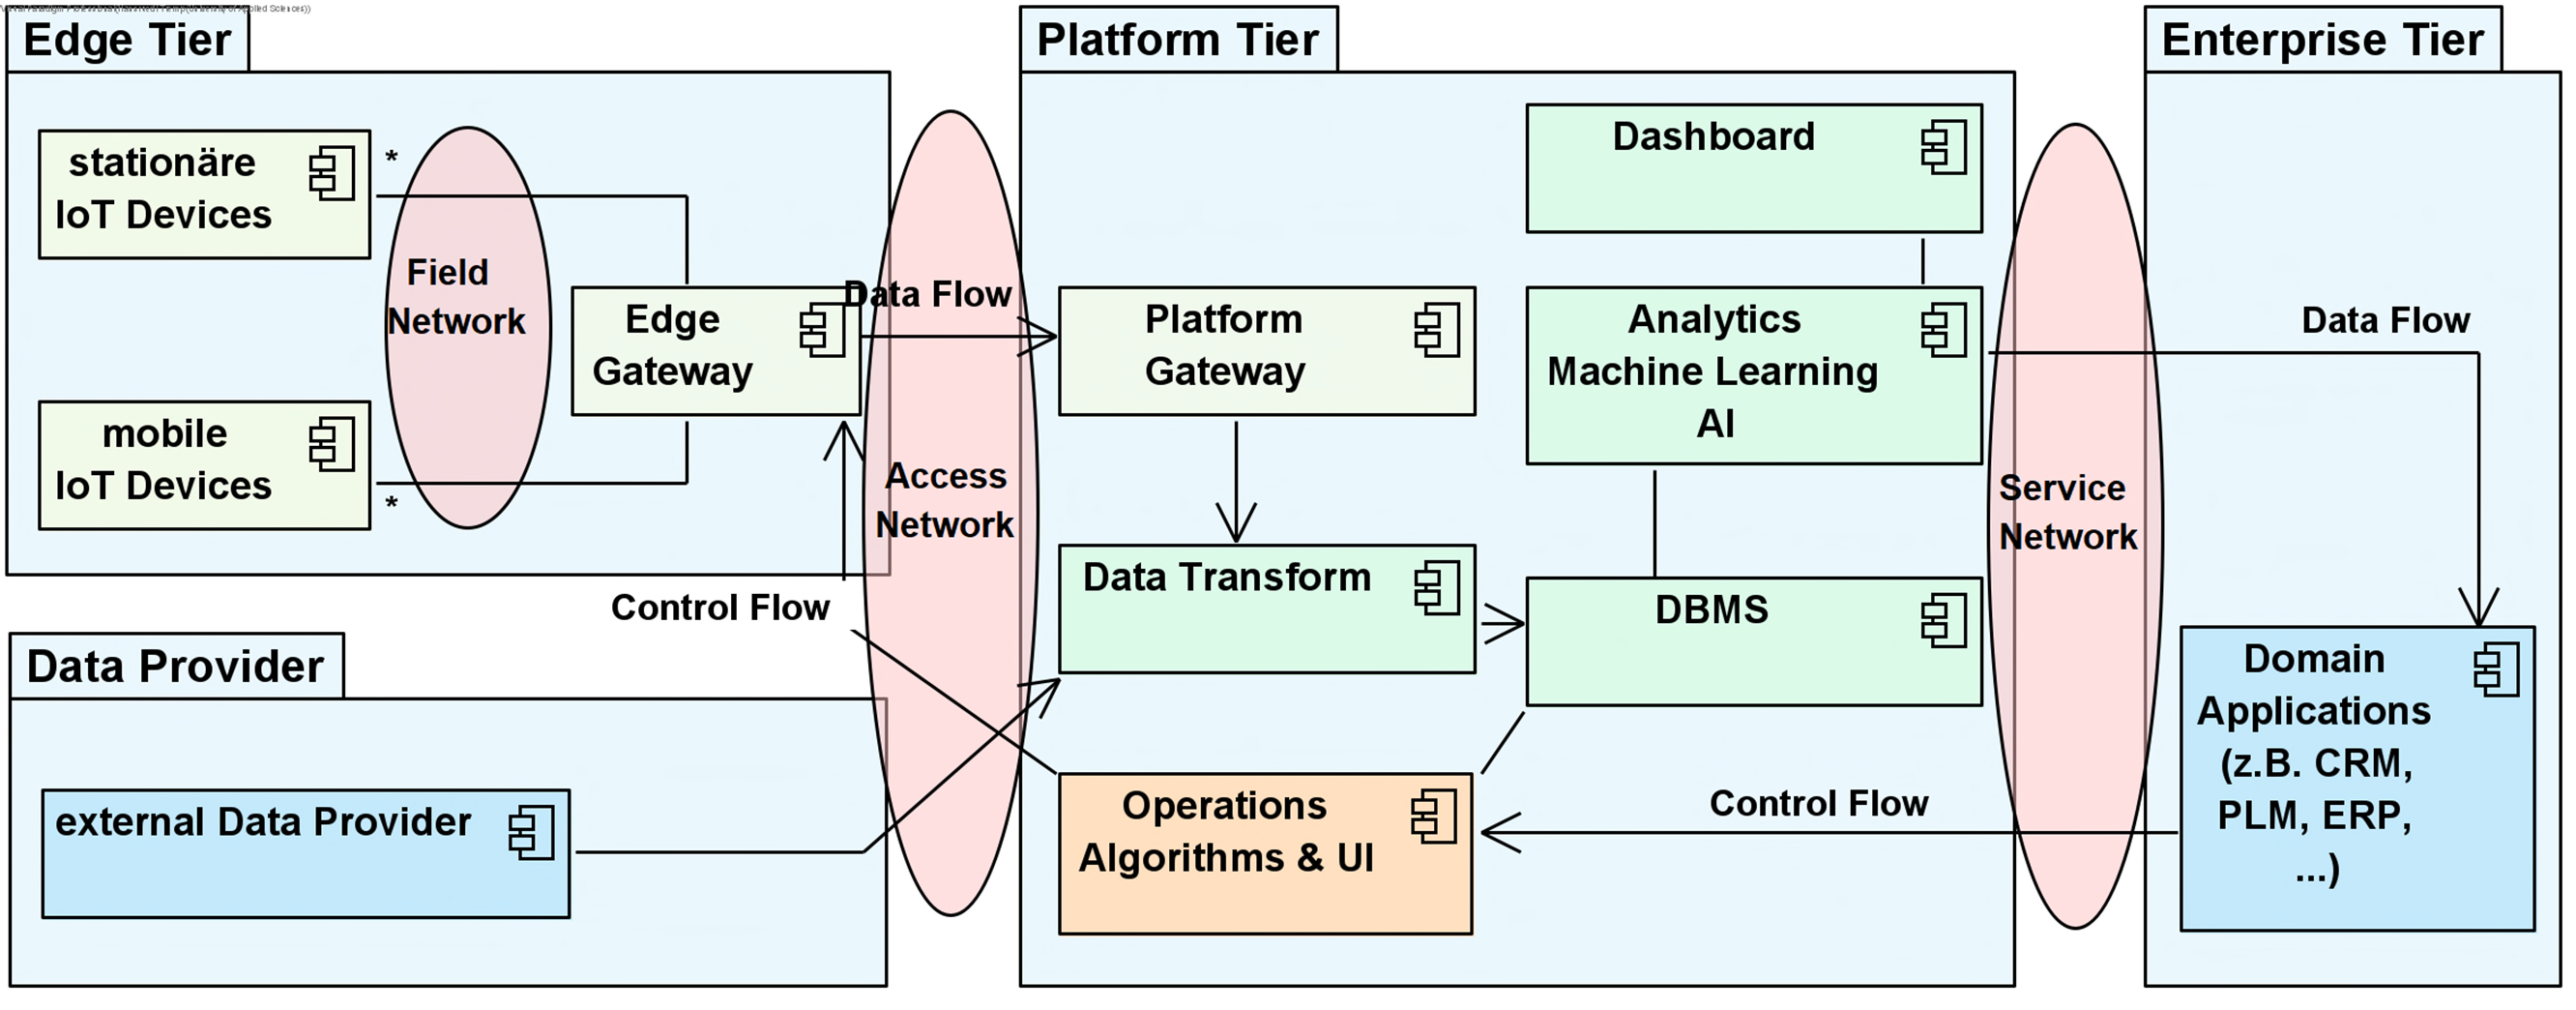
\includegraphics[width=\linewidth]{servers-iot-reference.png}

\begin{itemize}
    \item \textcolor{blue}{Edge Gateway} übernimmt Funktionen wie das Device Management, Security-Funktionen, Datenfilterung und Aggregation
    \item \textcolor{blue}{Platform Tier} lauft auf einem zentralen Server
    \item \textcolor{blue}{Data Transform} lädt aufbereitete Daten in das zentrale DBMS
    \item \textcolor{blue}{Dashboard} informiert berechtigte Stakeholder über aktuellen Stand
    \item \textcolor{blue}{Operationsmodul} enthält verschiedene Algorithmen zur Erzeugung von Seuerinformationen, welche zum Edge Gateway zurück fliessen
\end{itemize}
\vspace{10pt}
\textbf{Beispiel}

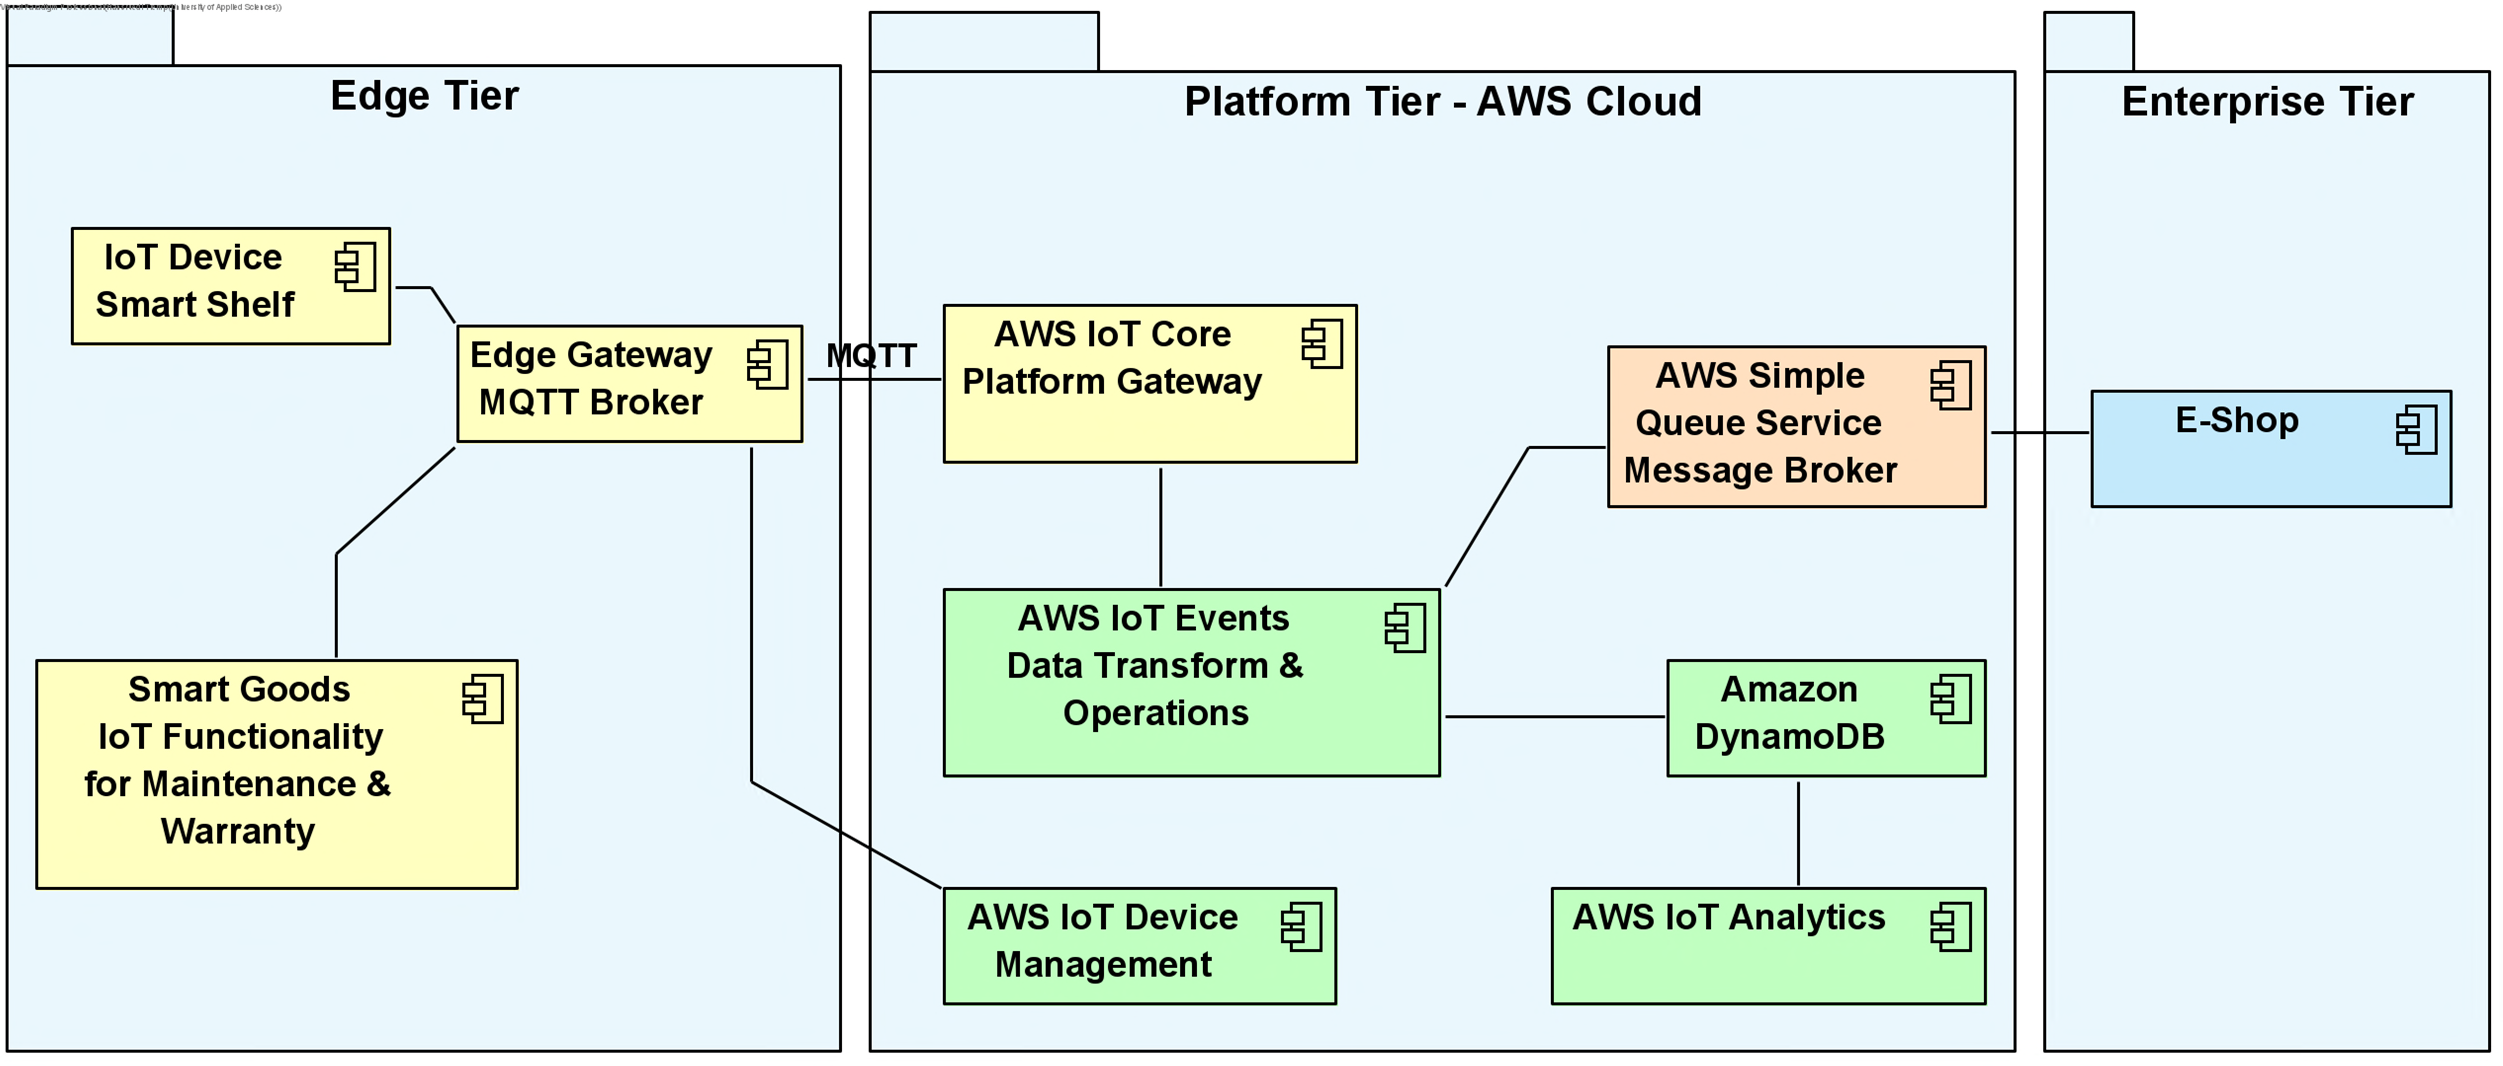
\includegraphics[width=\linewidth]{servers-iot-example.png}

\begin{itemize}
    \item Kunden verfügen über einen Smart Shelf
    \item Smart Goods sind mit IoT-Funktionalitäten ausgerüstet $\rightarrow$ Für den Unterhalt und die Einhaltung der Servicefenster während der Garantie sind diese mit dem Edge Gateway verbunden
    \item Edge Gateway tauscht Messages über MQTT mit AWS IoT Core aus
    \item AWS IoT Events nimmt Sensordaten entgegen und verarbeitet diese Referenzarchitektur
    \item Daten werden entweder in der DynamoDB gespeichert und/oder messages über den AWS
    Simple Queue Services Borker ausgetauscht
    \item Je nach Informationen löst der E-Shop Wartungshandlungen bzw. Bestellungen aus
\end{itemize}

\textbf{Cloud}

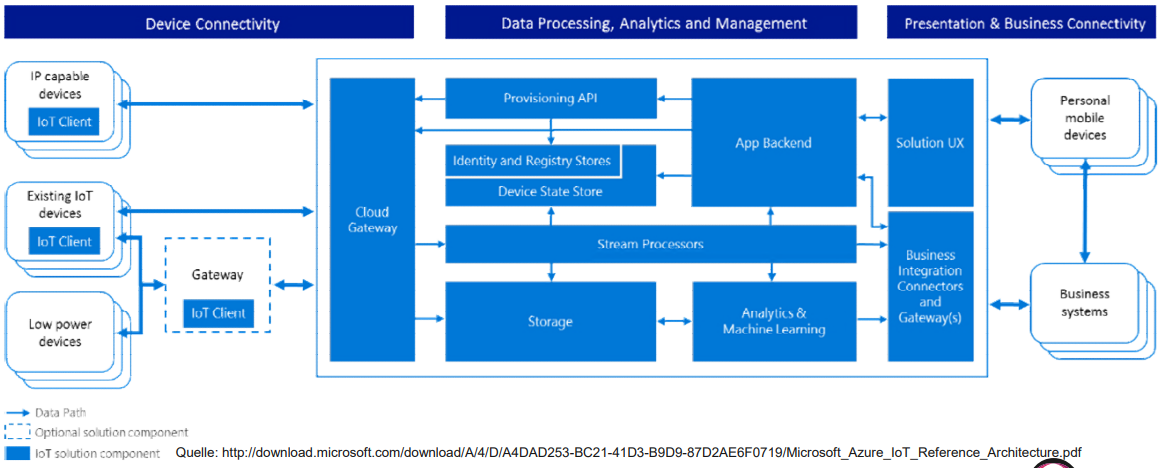
\includegraphics[width=\linewidth]{servers-iot-azure.png}

\subsubsection{Prüfungsfragen}

\begin{itemize}
    \item Welche Funktion übt der Service Tier aus? Welche drei Spezifikationen stehen Ihnen in Jakarta EE dafür zur Verfügung? \\
    \textcolor{blue}{Für Datenaustausch mit den Client und Umsystemen. JAX-WS, JAX-RS und JAX-RPC}
    \item In welchem Szenario in Bezug auf die Funktionalität der Applikation macht ein Business Workflow Tier Sinn? \\
    \textcolor{blue}{Wenn Kunden applikationsinterne Workflows benötigen}
    \item Inwiefern erhöht die für den Anwender frei definierbaren Geschäftsregeln die Flexibilität des Einsatzes einer Applikation? Wo sind deren Grenzen? \\
    \textcolor{blue}{Antwort}
    \item Auf welchen Plattformen (OS) laufen .NET 5-Applikationen? \\
    \textcolor{blue}{Windows, macOS und Linux}
    \item Skizzieren Sie eine .NET Mehrschichtenarchitektur mit einer ASP.NET MVC Client-App, einem Zugriff auf einen Payment Service Provider so wie der Verwendung des MS SQL-Servers \\
    \textcolor{blue}{Antwort}
    \item Wie verorten Sie die drei Begriffe: J2EE, Jakarta EE, Java EE 8 zeitlich und inhaltlich? Welche Organisation stand bzw. steht jeweils dahinter? \\
    \textcolor{blue}{J2EE $\rightarrow$ Sun (1999-2003), Java EE 8 $\rightarrow$ Oracle (2017), Jakarta EE $\rightarrow$ Eclipse Foundation (2019)}
    \item Wie unterscheidet sich der Aufbau des Middle Tier in .NET gegenüber Jakarta EE? \\
    \textcolor{blue}{Siehe dessen Referenzarchitekturen}
    \item Beschreiben Sie die Stationen des Datenflusses ausgehend von Sensor-Daten in einem IoT Device, welche letztendlich dazu führen, dass das PLM (Product Lifecycle Management) neue Anweisungen für die Aktuatoren sendet \\
    \textcolor{blue}{Edge Gateway $\rightarrow$ Platform Gateway $\rightarrow$ Analytics Machine Learning AI $\rightarrow$ Domain Applications}
\end{itemize}
